\chapter{Introdução}\label{cap_introducao}

\section{Problemas de Otimização}

Em matemática e ciência da computação, problemas de otimização consistem naqueles em que
a solução é um elemento de um conjunto de candidatos que melhor satisfaz uma determinada
série de condições. Um exemplo clássico dessa classe é o problema da mochila 
(\textit{knapsack problem}, em inglês), no qual
procura-se, dentre um conjunto de itens com diversos preços e pesos, o subconjunto que
maximiza o valor total. Esse valor é calculado somando-se os preços dos itens postos na
mochila. 

Entretanto a solução deve respeitar um vínculo: o peso total dos objetos escolhidos
não deve exceder o peso máximo suportado pela mochila. Ainda que seja possível encontrar a solução exata
desse problema usando algoritmos de programação dinâmica,
a complexidade de tais algoritmos é $ \mathcal{O} (n w) $, onde $n$ é o número de itens e $w$ é a
capacidade da bolsa. Assim, o tempo de execução para muitos itens\trav que é o caso de interesse,
usualmente\trav pode ser mais longo do que o desejado.

Outro exemplo comum de problema de otimização é o de otimização numérica, do qual constituem
solução os pontos de máximo ou mínimo global de uma função 
$ f : \R^m \rightarrow \R $. Tomemos como exemplo simples a função
\begin{equation}
  f(x, y) = \cos(n\pi r)\exp\left(-\frac{r^2}{\sigma^2}\right) \mathcomma
  \label{eq:damped_cos}
\end{equation}
definida no domínio $ [-1, 1] \times [-1, 1] $, cujo gráfico se encontra na Figura \ref{fig:damped_cos}.
Os parâmetros $n$ e $\sigma$ são reais, e modificam a frequência de oscilação da função e a rapidez
de decaimento da amplitude, respectivamente.
Analiticamente é fácil determinar o ponto de máximo global em $ r = 0 $ usando métodos de cálculo
para funções de múltiplas variáveis. 
Contudo, não é sempre que pode-se dispor de tal facilidade. 
Nos casos em que a função objetivo é de maior complexidade, com domínio contido em espaços de maior dimensão; 
em que a função tem evolução temporal; em que a função possui diversas descontinuidades; ou em que a função
depende de variáveis aleatórias, o problema se torna impraticável de resolver de forma analítica. 
Isto posto, como desenvolver um algoritmo para encontrar a solução?

\begin{figure}
  \centering
  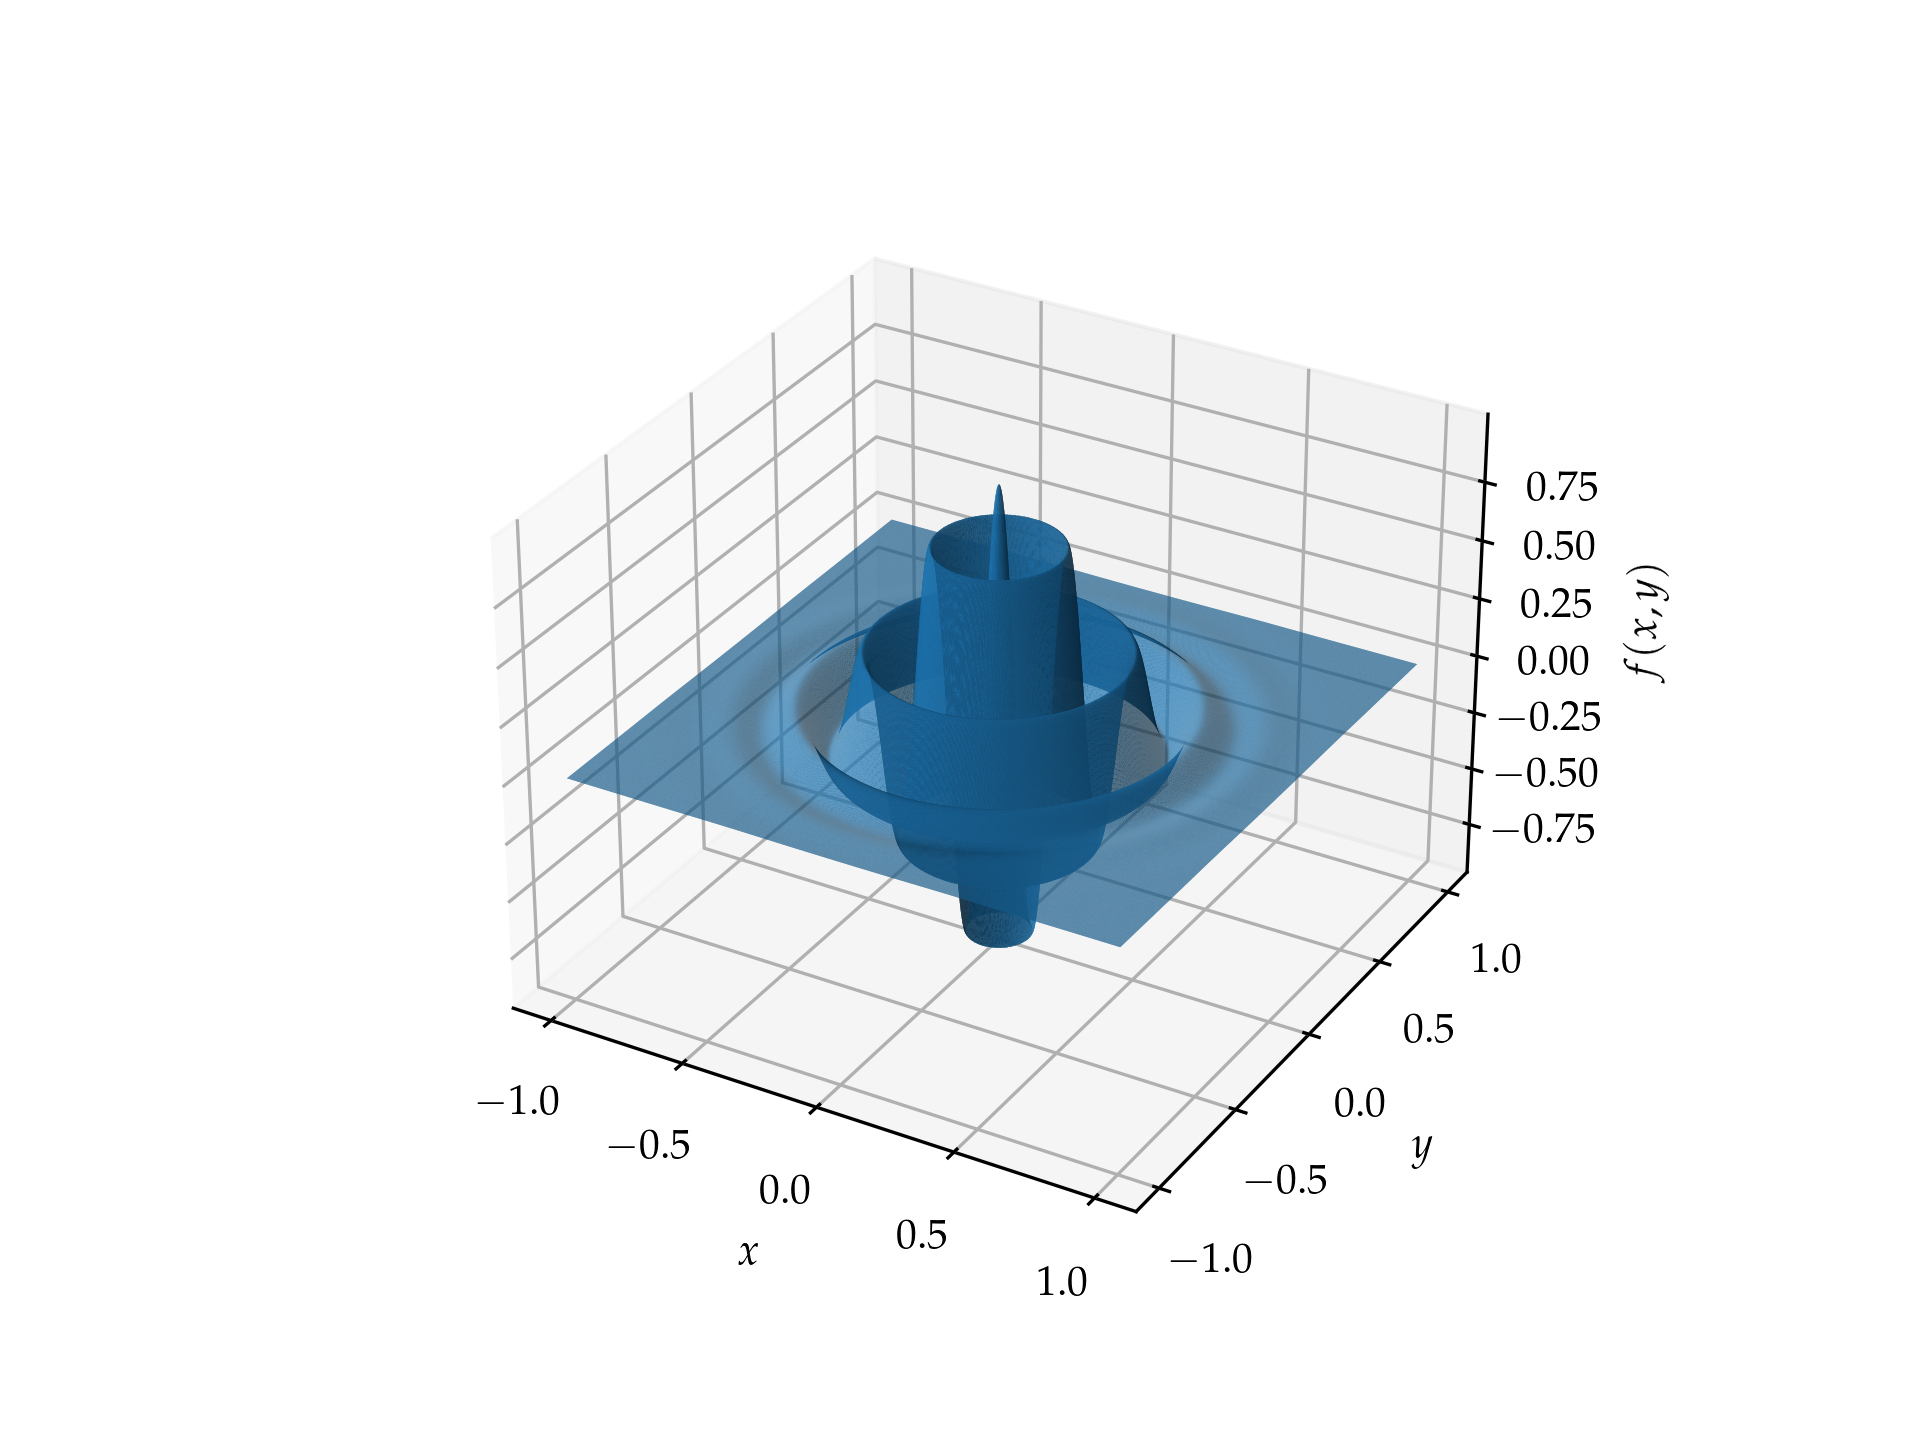
\includegraphics[width=\textwidth]{imagens/damped_cossine.png}
  \caption{Gráfico da função definida na Equação \ref{eq:damped_cos}, com $ n = 9 $ e $ \sigma = 0,4 $.}
  \label{fig:damped_cos}
\end{figure}

Uma classe de algoritmos mais simples que se propõem a resolver esse problema são os algoritmos do
tipo escalada de morro (\textit{hill climbing}, em inglês). 
Sugerido pelo nome, o funcionamento desses algoritmos consiste, resumidamente,
em sortear um ponto inicial no domínio da função, calcular o gradiente da função no ponto, e seguir
na direção resultante por uma distância pré-definida, e repetir esses passos até que o módulo do
vetor gradiente seja próximo de zero, respeitando uma tolerância previamente determinada  \cite{goldberg1989ga}. 

O problema com esse tipo de algoritmo é que, quando aplicado em funções como a definida anteriormente, a tendência é
de que a solução encontrada seja um máximo local na grande maioria das vezes. No caso da função definida
pela Equação \ref{eq:damped_cos}, o máximo global só seria encontrado pelo algoritmo se o ponto inicial
ocorresse na região delimitada pelo primeiro mínimo local, isto é, na região\footnote{
  Tal probabilidade é computada tomando a razão entre a área delimitada pelo primeiro mínimo local
  e a área total do domínio em questão.
}
tal que $ r < \nicefrac{1}{n} $. 
Se os pontos iniciais do algoritmo forem gerados aleatoriamente,
para o domínio definido, a probabilidade de um ponto pertencer a esta região é $ P(n) = \nicefrac{\pi}{4n^2} $.
Para $ n = 9 $, como na Figura \ref{fig:damped_cos}, $ P \approx 1\% $. 
Ademais, é possível que esse tipo
de algoritmo indique erroneamente como solução pontos de sela e planícies em determinados casos, o que o
torna ainda menos eficaz para o propósito.

Uma outra categoria de algoritmos que podem resolver ambos os problemas de forma rápida e chegar a uma
solução que se aproxima o suficiente da solução exata são os algoritmos genéticos. Tais algoritmos,
quando bem implementados, podem chegar a uma solução aproximada para o problema da mochila de forma
rápida para valores de $n$ e $w$ ordens de grandeza superiores aos que tornariam praticável o uso da
estratégia proposta anteriormente. 

No problema de otimização numérica, um algoritmo desse tipo é vantajoso pois é capaz de chegar na solução
de forma rápida na maioria dos casos, identificando não só o máximo global, como também os máximos
locais contidos na região de busca. Outra vantagem é que esse método pode ser aplicado sem problemas
em espaços de busca com grande número de dimensões, ou em funções não estacionárias, contínuas ou
descontínuas. Além disso, como será mostrado posteriormente, o algoritmo é paralelizável, o que pode
acelerar a obtenção de uma solução.

\section{O Algoritmo Genético}

Os algoritmos genéticos foram primeiramente desenvolvidos por John Henry
Holland \cite{holland1992ga} na década de 60. Levam esse nome pois sua formulação teve como 
forte influência o processo de evolução natural que fomenta a origem das espécies desde o surgimento da vida
em nosso planeta. Em sua execução, é inicializada uma população de indivíduos da mesma espécie\footnote{
  Isso significa que seus respectivos códigos genéticos possuem a mesma estrutura: mesma número de
  cromossomos com uma mesma quantidade de genes. Assim, pode haver reprodução entre tais indivíduos.
}.
Cada indivíduo corresponde a um candidato a solução do problema de otimização proposto, e tem sua
identidade codificada pelo seu material genético\footnote{
  No caso do problema da mochila, por exemplo, uma
  estrutura natural para o material genético é um cromossomo binário, com $n$ genes, cada um correspondente
  a um objeto do problema. Por outro lado, no problema de otimização numérica, dois cromossomos seriam
  necessários, um para codificar cada coordenada em cada dimensão do espaço de busca.
}.
Então, sob algum critério, é selecionada uma parcela desses indivíduos, a qual dará origem a novos
descendentes, cujos cromossomos serão gerados pela recombinação dos cromossomos correspondentes nos
pais. Nesse passo é introduzida uma probabilidade de mutação nos genes dos filhos. 

Ao final desse processo, descarta-se a parcela não selecionada da população, dando origem a uma nova geração, formada
pelos pais e seus filhos. Esse processo é repetido iterativamente até que uma condição de parada seja
atingida. Essa condição pode ser imposta sobre o número de gerações ou sobre o tempo de execução do programa.
Pode ainda ocorrer quando for observado uma determinada característica na população, persistente no decorrer das gerações,
No caso de um problema de otimização numérica, a observação de uma porção de indivíduos com seus genes
constantes durante um número grande de gerações pode significar a convergência dessa parcela da população
para um máximo global, por exemplo.
Respeitando as diferenças de implementação em cada passo, devido as peculiaridades de cada tipo de problema
de otimização proposto, essas etapas são presentes em todo algoritmo genético, e são bem resumidas no fluxograma
presente na Figura \ref{fig:ga_flow}.

\begin{figure}
  \centering
  \begin{tikzpicture}
    \node[start_end] (start) {Início};
    \node[io, below=1em of start] (init_pop) {População\\ Inicial};
    \node[process, below=1em of init_pop]  (selection) {Seleção};
    \node[process, below=1em of selection]  (crossover) {Recombinação};
    \node[process, below=1em of crossover]  (mutation) {Mutação};
    \node[decision, below=1em of mutation]  (check) {Condição atingida?};
    \node[document, left=10ex of check] (print_stats) {Informações da\\População};
    \node[start_end, above=10ex of print_stats] (end) {Fim};
    \draw[myarrow=.9] (start.south) --  (init_pop.north);
    \draw[myarrow=.9] (init_pop.south) --  (selection.north);
    \draw[myarrow=.9] (selection.south) --  (crossover.north);
    \draw[myarrow=.9] (crossover.south) --  (mutation.north);
    \draw[myarrow=.9] (mutation.south) -- (check.north);
    \draw[myarrow=.9] (check.east) -- node[description, above] {Não} ([xshift=10ex]check.east) |- (selection.east);
    \draw[myarrow=.9] (check.west) -- node[description, above] {Sim} (print_stats.east);
    \draw[myarrow=.9] (print_stats.north) -- (end.south);
  \end{tikzpicture}
  \caption{Fluxograma geral de um algoritmo genético.}
  \label{fig:ga_flow}
\end{figure}

\section{Um Exemplo Físico: Ajuste das Estruturas de Banda de Dicalcogenetos de Metais de Transição}
\label{sec_tmdcs_intro}

Dicalcogenetos de metais de transição (TMDC, do inglês 
\textit{transition-metal dichalcogenides}) são materiais cuja composição é
descrita por \ch{MX2}, sendo \ch{M} um metal de transição e \ch{X} um calcogênio
(\ch{S}, \ch{Se} ou \ch{Te}). São conhecidos cerca de 60 compostos de tal classe,
dos quais cerca de 20 apresentam estrutura cristalina na forma de finas camadas, com
espessuras na ordem de $10\si{\angstrom}$ \cite{kolobov2016tmdc}. Por essa razão, 
podem ser categorizados como materiais bidimensionais.

A maioria desses materiais são sintéticos, mas alguns podem ser encontrados na natureza,
como \ch{MoS2}\trav dissulfeto de molibdênio\trav que ocorre naturalmente na
forma do mineral molibdenita, sendo esse a principal fonte de obtenção do molibdênio.
Uma fotografia desse mineral, bem como uma representação de sua estrutura cristalina
são ilustrados na Figura \ref{fig:mos2}.

\begin{figure}[ht]
  \begin{subfigure}{0.49\textwidth}
    \centering
    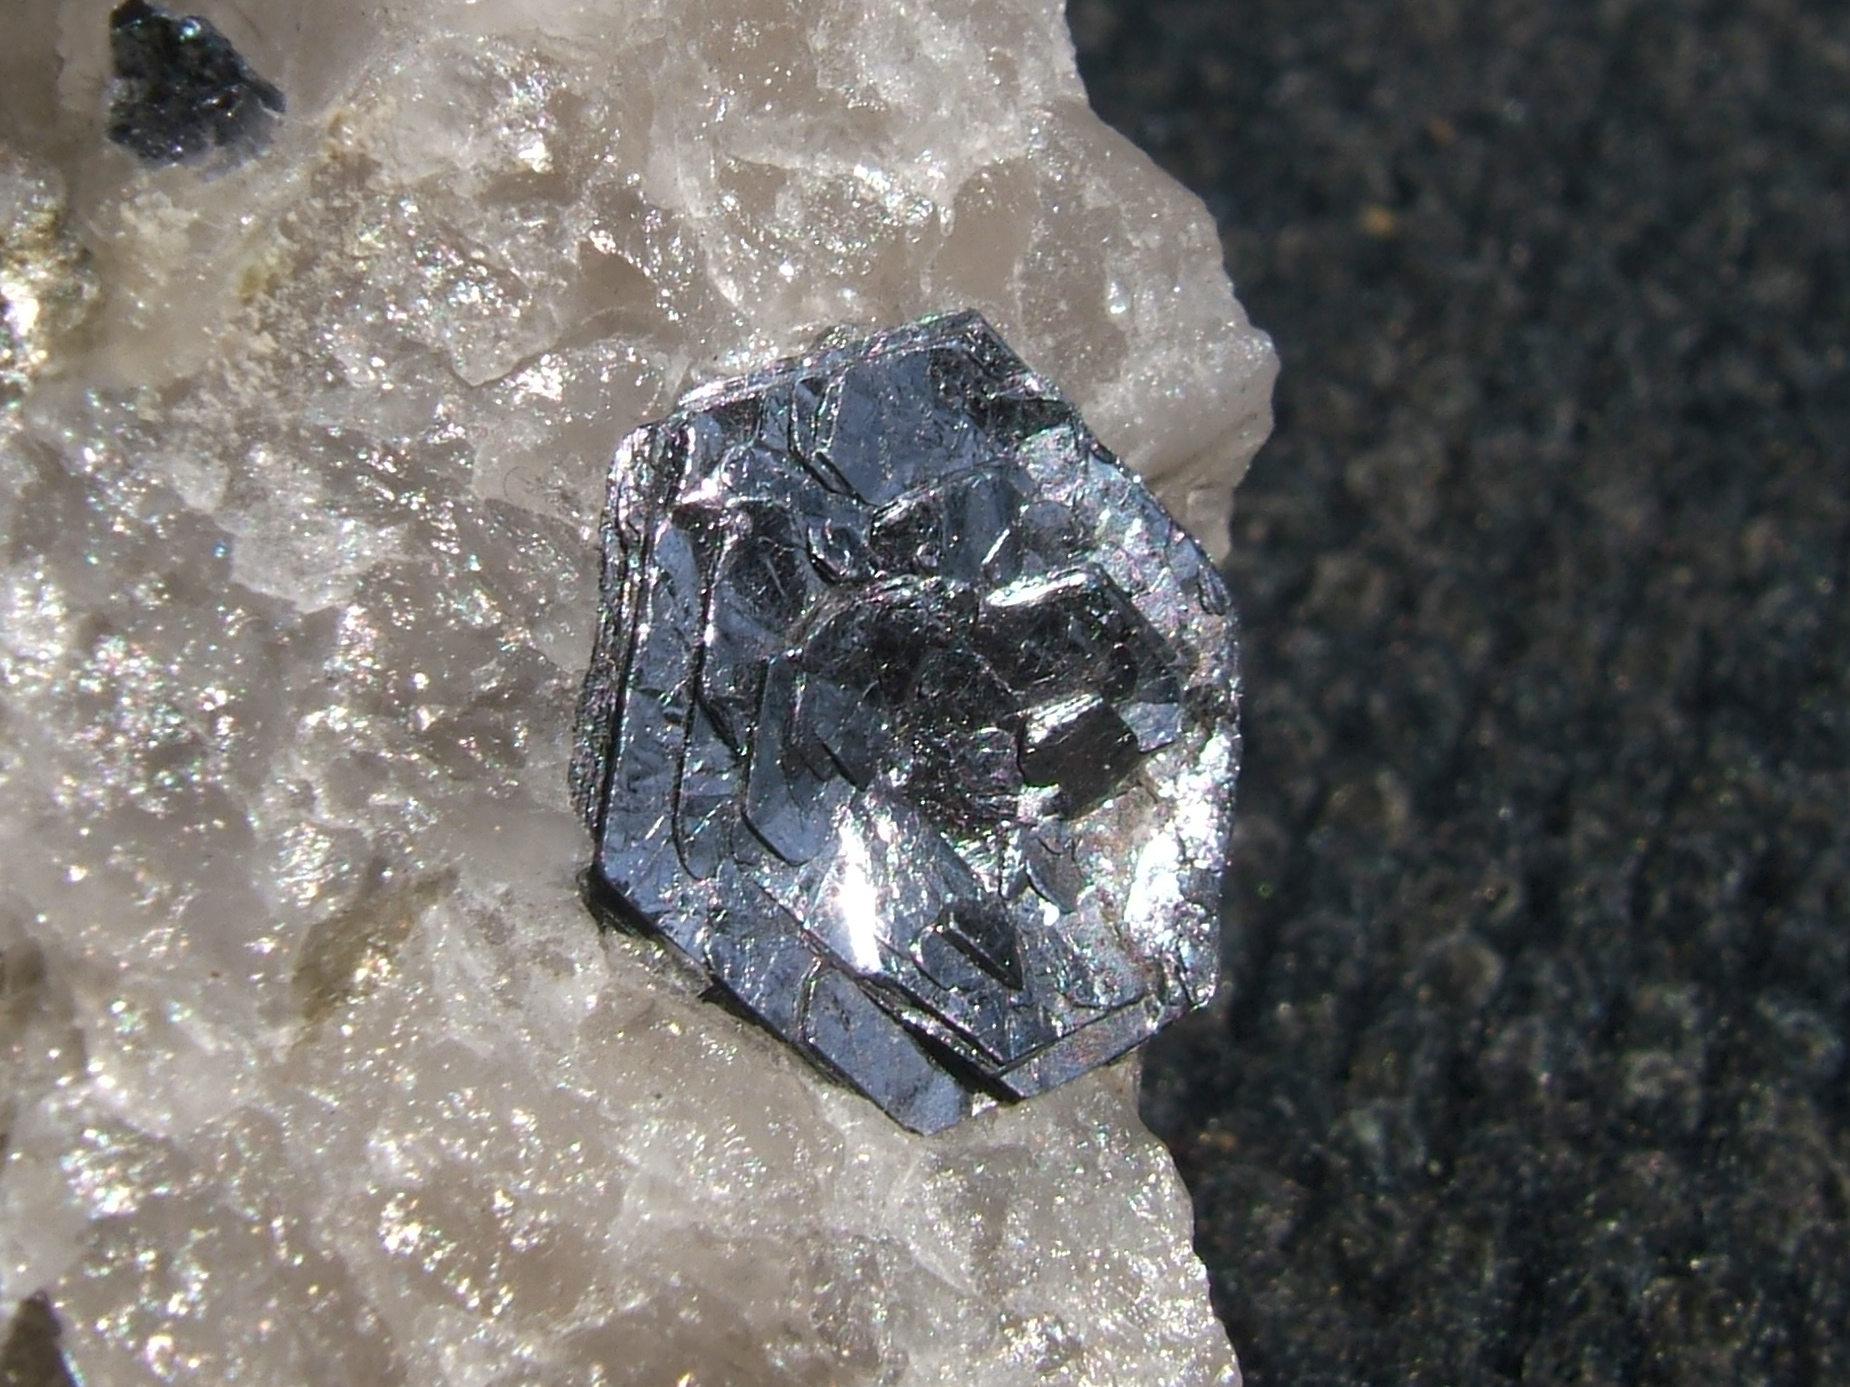
\includegraphics[width=1.0\linewidth]{imagens/molybdenite.jpeg}
    \caption{}
    \label{fig:mos2a}
  \end{subfigure}
  \begin{subfigure}{0.49\textwidth}
    \centering
    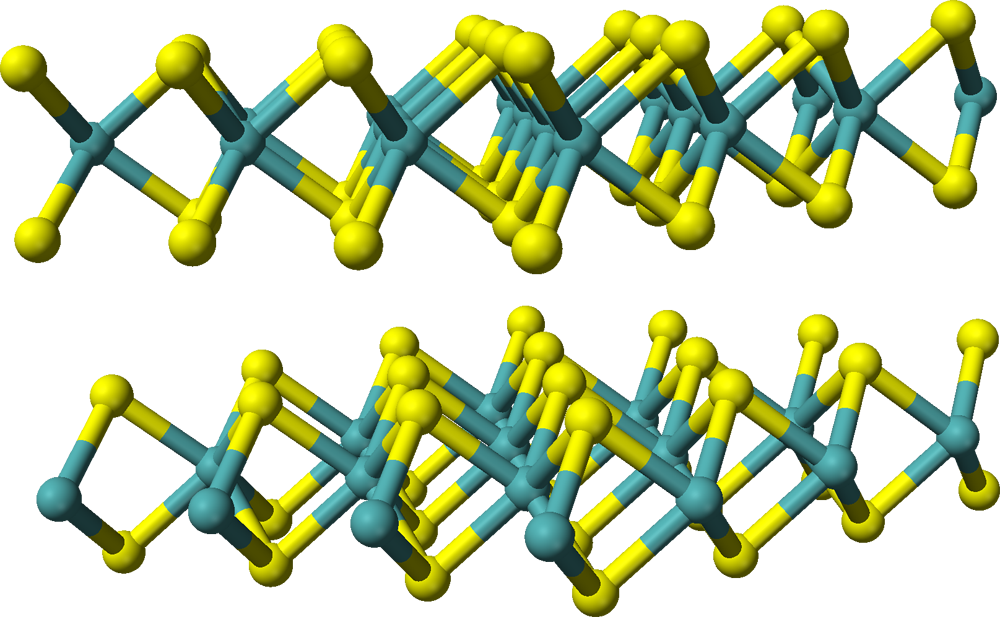
\includegraphics[width=1.0\linewidth]{imagens/molybdenite_crystal.png}
    \caption{}
    \label{fig:mos2b}
  \end{subfigure}
  \caption{
    \subref{fig:mos2a} Molibdenita incrustada em uma massa de quartzo.
    \subref{fig:mos2b} Representação da estrutura cristalina da molibdenita. Molibdênio em azul, enxofre em amarelo.
  }
  \label{fig:mos2}
\end{figure}

\newcommand\xsla{-1.2}
\newcommand\ysla{0.505}
\newcommand\hexheight{3em}
\newcommand\hexside{2em}

\newcommand\hex[3][]{
  \begin{scope}[
      #1,
      xscale=-1,
      yshift=#3,
      yslant=\ysla,
      xslant=\xsla,
      every node/.style={anchor=west,regular polygon,regular polygon sides=6,draw,inner sep=\hexside},
      transform shape
    ]
    \node (hex_#2) {};
  \end{scope}
}

\newcommand\hexhidden[3][]{
  \begin{scope}[
      #1,
      xscale=-1,
      yshift=#3,
      yslant=\ysla,
      xslant=\xsla,
      every node/.style={anchor=west,regular polygon,regular polygon sides=6,inner sep=\hexside,draw,dotted},
      transform shape
    ]
    \node (hex_#2) {};
  \end{scope}
}

\begin{figure}[b]
  \centering
  \begin{tikzpicture}
    \hex{top}{\hexheight}
    \hexhidden{middle}{0}
    \hex{bottom}{-\hexheight}

    \foreach \corn in {1,...,6}
    \draw (hex_top.corner \corn) -- (hex_bottom.corner \corn);

    % Caminho no qual as bandas são calculadas
    \draw[thick,myarrow=0.5] (hex_middle.center) -- (hex_middle.corner 4);
    \draw[thick,myarrow=0.5] (hex_middle.corner 4) -- (hex_middle.side 3);

    % Pontos de simetria
    \draw[fill=black] (hex_middle.center) circle (2pt) node[right]{$\Gamma$};
    \draw[fill=black] (hex_middle.corner 4) circle (2pt) node[below left]{$K$};
    \draw[fill=black] (hex_middle.side 3) circle (2pt) node[below right]{$M$};
    \draw[fill=black] (hex_middle.corner 3) circle (2pt) node[above right]{$K'$};
    \draw[fill=black] (hex_top.center) circle (2pt) node[above right]{$A$};
  \end{tikzpicture}
  \caption{
    Zona de Brillouin para monocamadas de TMDCs e principais pontos de simetria.
    Geralmente as bandas de valência e de condução são calculadas ao longo desses
    pontos, como no caminho exemplificado.
  }
  \label{fig:brillouin}
\end{figure}

Esses materiais voltaram a ser amplamente estudados com a descoberta recente das
propriedades eletrônicas do grafeno, pela qual K. S. Novoselov e A. K. Geim foram
condecorados com o prêmio Nobel em 2010 \cite{kolobov2016tmdc}. Assim como no caso do grafeno, alguns
TMDCs são semicondutores, característica essa que possibilita um grande leque de
aplicações na indústria. 

Dentre tais aplicações se destacam a manufatura de transistores, circuitos
lógicos e amplificadores. Ademais, a estrutura eletrônica de alguns TMDCs torna
propícia a formação de excitons em sua estrutura cristalina, o que abre margem
para aplicações em dispositivos optoeletrônicos, como fotodetectores e células
solares.

Em todos esses casos é de fundamental importância que se tenha conhecimento
acerca dos níveis de energia do sólido em questão. Em particular, é de interesse
prático o cálculo dos níveis de energia das bandas de valência e de
condução\trav último nível de energia ocupado e primeiro nível de energia não
ocupado, respectivamente. Desses valores se calcula a energia necessária para a
formação de excitons\footnote{
  Um exciton é um par elétron-buraco formado pela transição de um elétron de
  valência para uma camada de condução. Em alguns sólidos e moléculas pode haver o
  transporte de excitons, fenômeno explorado semicondutores no geral. 
}, o que é determinante na confecção dos dispositivos optoeletrônicos enumerados
no parágrafo anterior. Esse valor é conhecido como o \textit{bandgap} do material.

Existe uma área na engenharia\trav denominada engenharia de
\textit{gap}\trav dedicada à manufatura de materiais com propriedades
eletrônicas específicas, as quais são obtidas por meio do controle deste valor
por intermédio de diversas técnicas. Um exemplo é o \textit{doping}, que
consiste a introdução de átomos distintos à composição do material em sua rede
cristalina, aplicada com frequência na fabricação de diodos e transistores
usados nos mais diversos dispositivos eletrônicos.

Usualmente, calcula-se tais bandas ao longo da primeira zona de Brillouin do
cristal, a qual é a correspondente da célula primitiva no espaço recíproco\footnote{
  Resumidamente, o espaço recíproco pode ser visto como  o espaço gerado 
  pela transformada de Fourier dos vetores primitivos, os quais constituem
  a chamada célula unitária, e por conseguinte, descrevem a estrutura 
  cristalina de um sólido.
}. Para
o caso dos matérias em questão, a zona de Brillouin é do tipo hexagonal, e se
encontra ilustrada ná Figura \ref{fig:brillouin}, conjuntamente aos principais
pontos de simetria. Desses pontos de alta simetria, $K$ e $K'$ coincidem com os
mínimos locais do \textit{bandgap} do sistema, e por isso são de maior
relevância.

Um dos métodos mais utilizados para o cálculo das bandas é a Teoria do Funcional
Densidade (DFT, do inglês \textit{density-functional theory}), o qual é um
modelo quântico computacional para a aproximação das soluções de sistemas
quânticos com múltiplas partículas, amplamente utilizado na química e na física,
particularmente em física do estado sólido e física da matéria condensada.

\begin{figure}[h]
  \centering
  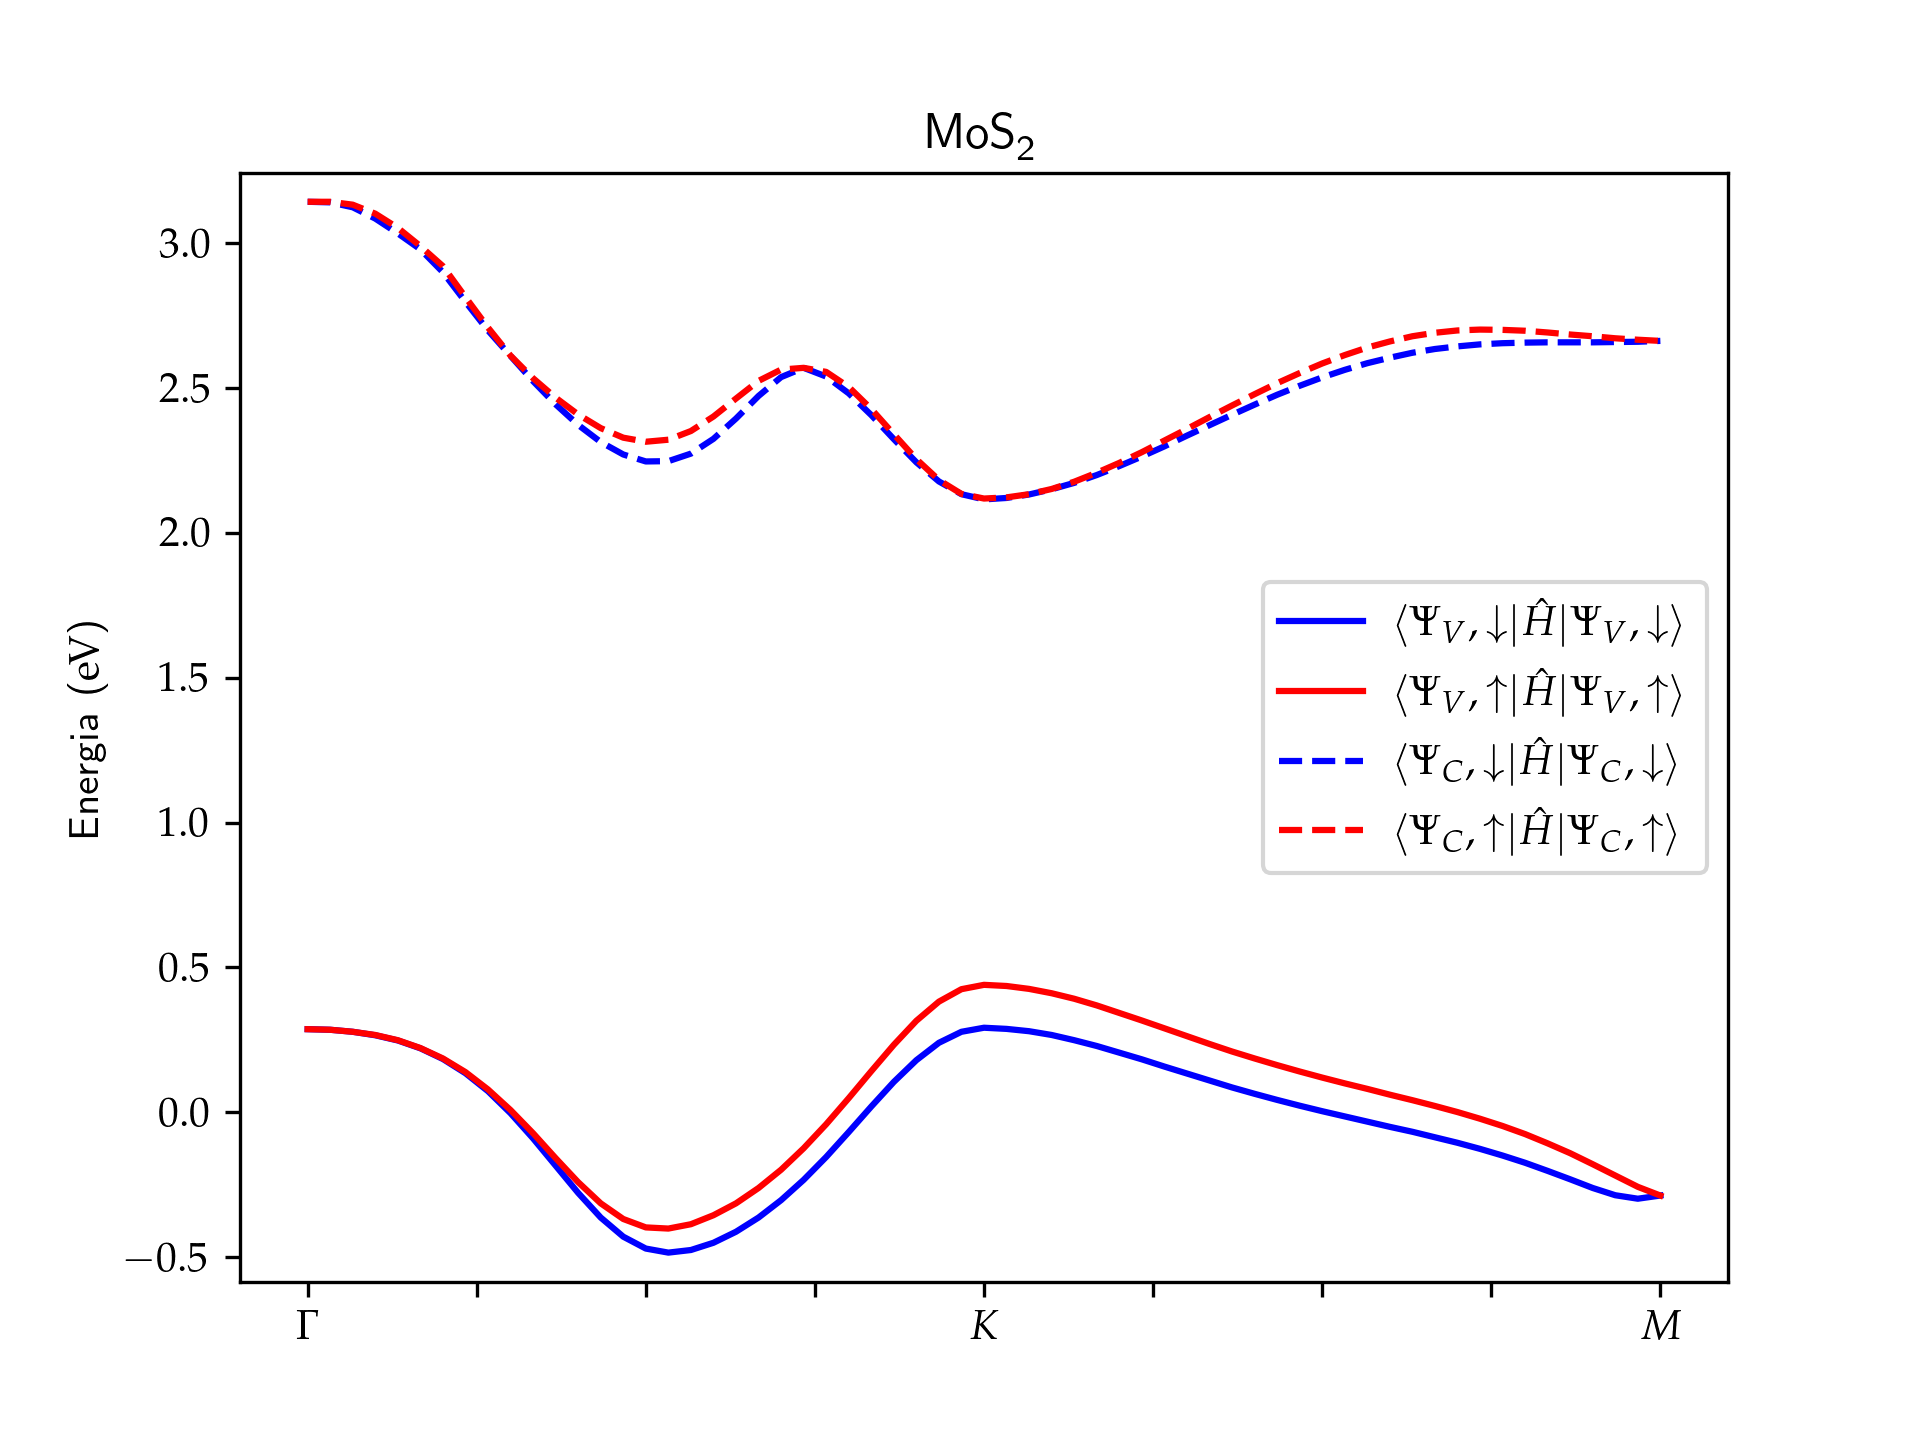
\includegraphics[width=\textwidth]{imagens/mos2_bands.png}
  \caption{
    Energias das bandas de condução e de valência ao longo do caminho ilustrado
    na Figura \ref{fig:brillouin} para o dissulfeto de molibdênio.
  }
  \label{fig:mos2_bands}
\end{figure}

No entanto, existem outros modelos para a estimativa das bandas de condução e de
valência, como o modelo $k \cdot p$\trav também conhecido como modelo de baixas
energias, descrito em \cite{liu2013tmdc}\trav o qual se propõe a aproximar essas
bandas em torno de $K$ ou $K'$.

Das vantagens do uso desse modelo pode-se destacar o fato de ser um modelo
aproximativo analítico, o que facilita o desenvolvimento de uma intuição física
acerca do material, possibilitando a observação do comportamento das bandas de
energia com a variação dos parâmetros que as descrevem. Também trata-se de um
modelo computacionalmente barato, possibilitando a aproximação de sistemas que
seriam computacionalmente complexos quando estimados com o uso do método DFT.
Outra vantagem que será explorada subsequentemente na seção
\ref{sec_resultados_tmdcs} é a possibilidade da inclusão de um campo magnético
normal à monocamada do TMDC à descrição do sistema graças à existência de uma
forma analítica para a hamiltoniana do cristal, o que tornaria impraticável
o uso do método DFT.

No modelo $ k \cdot p $ a hamiltoniana na representação da base
\begin{equation}
  \left\{ \ket{\Psi_C,\uparrow} ; \ket{\Psi_C,\downarrow} ; \ket{\Psi_V,\uparrow} ; \ket{\Psi_V,\downarrow} \right\}
  \label{eq:basis}
\end{equation}
é escrita na forma
\begin{equation}
  \hat{H}_{kp}(\bvec{k}) = \hat{H}_0 + \sum_{i=1}^3 \hat{H}_{kp}^{(i)}(\bvec{k})
  \label{eq:total_ham}
\end{equation}
onde $ \Psi_C $ e $ \Psi_V $ são as funções de onda do sistema com o elétron de
valência em sua camada original e na camada de condução, respectivamente e 
$ \hat{H}_{kp}^{(i)}(\bvec{k}) $ corresponde ao termo de ordem $ i $ com respeito
a $ \bvec{k} = (k_x, k_y, k_z) $, um ponto do espaço recíproco. 

Normalmente o vetor $ \bvec{k} $ é escrito em uma base $ \{\bvec{e}_x,\bvec{e}_y,\bvec{e}_z\} $
tal que $\Gamma$ se encontra na origem,
$ \bvec{e}_2 = \nicefrac{\bvec{K}'}{|\bvec{K}'|} $, 
$ \bvec{e}_3 = \nicefrac{\bvec{A}}{|\bvec{A}|} $ e 
$ \bvec{e}_1 = \bvec{e}_2 \times \bvec{e}_2 $, sendo 
$ \bvec{K}' $ e $ \bvec{A} $ os vetores que localizam os pontos de simetria $K'$ e $A$, respectivamente.
No entanto, nesse modelo é necessário aplicar uma translação em tal base tal que
a origem passe a ser localizada em $K$.

Os termos da expansão da hamiltoniana em função de $ \bvec{k} $ são dados por
\begin{align}
  \begin{split}
    &\hat{H}_0 =
    \left(
    \begin{matrix}
        E_F + \Delta - \tau \lambda_c & 0                         & 0                             & 0                         \\
        0                             & E_F + \tau \eta \lambda_v & 0                             & 0                         \\
        0                             & 0                         & E_F + \Delta + \tau \lambda_c & 0                         \\
        0                             & 0                         & 0                             & E_F - \tau \eta \lambda_v \\
      \end{matrix}
    \right) \\
    &\hat{H}_{kp}^{(1)}(\bvec{k}) =
    \left(
    \begin{matrix}
        0                                     & \gamma_0 f_1(\bvec{k},\tau) & 0                                     & 0                           \\
        \gamma_0 f_1^{\dagger}(\bvec{k},\tau) & 0                           & 0                                     & 0                           \\
        0                                     & 0                           & 0                                     & \gamma_0 f_1(\bvec{k},\tau) \\
        0                                     & 0                           & \gamma_0 f_1^{\dagger}(\bvec{k},\tau) & 0                           \\
      \end{matrix}
    \right) \\
    & \hat{H}_{kp}^{(2)}(\bvec{k}) =
    \left(
    \begin{matrix}
        \gamma_1 f_2(\bvec{k})                & \gamma_3 f_3(\bvec{k},\tau) & 0                                     & 0                           \\
        \gamma_3 f_3^{\dagger}(\bvec{k},\tau) & \gamma_2 f_2(\bvec{k})      & 0                                     & 0                           \\
        0                                     & 0                           & \gamma_1 f_2(\bvec{k})                & \gamma_3 f_3(\bvec{k},\tau) \\
        0                                     & 0                           & \gamma_3 f_3^{\dagger}(\bvec{k},\tau) & \gamma_2 f_2(\bvec{k})      \\
      \end{matrix}
    \right) \\
    &\hat{H}_{kp}^{(3)}(\bvec{k}) =
    \left(
    \begin{matrix}
        \gamma_4 f_4(\bvec{k})                & \gamma_6 f_5(\bvec{k},\tau) & 0                                     & 0                           \\
        \gamma_6 f_5^{\dagger}(\bvec{k},\tau) & \gamma_5 f_4(\bvec{k})      & 0                                     & 0                           \\
        0                                     & 0                           & \gamma_4 f_4(\bvec{k})                & \gamma_6 f_5(\bvec{k},\tau) \\
        0                                     & 0                           & \gamma_6 f_5^{\dagger}(\bvec{k},\tau) & \gamma_5 f_4(\bvec{k})      \\
      \end{matrix}
    \right)
  \end{split}
\end{align}
sendo $E_F$ a energia do nível de Fermi; $\Delta$ o \textit{bandgap} do sistema;
$\lambda_c$ e $\lambda_v$ os termos de acoplamento spin-órbita nos níveis de
condução e valência, respectivamente; $\eta$ um índice referente ao metal de
transição em questão; $\tau$ o índice de vale, sendo $ \tau = 1 $ correspondendo
ao vale em $K$, e $ \tau = -1 $ correspondendo ao vale em $K'$ e $ \gamma_i $
são parâmetros de energia, os quais governam propriedades óticas do cristal. 
As funções $f_i$ são dadas pelas expressões
\begin{align}
  \begin{split}
    & f_1(\bvec{k},\tau) = a(\tau k_x - i k_y)                    \\
    & f_2(\bvec{k}) = a^2(k_x^2 + k_y^2)                          \\
    & f_3(\bvec{k},\tau) = a^2(\tau k_x + i k_y)^2                \\
    & f_4(\bvec{k},\tau) = a^3 \tau k_x (k_x^2 - 3 k_y^2)         \\
    & f_5(\bvec{k},\tau) = a^3 (k_x^2 + k_y^2) (\tau k_x - i k_y)
  \end{split}
\end{align}
onde $a$ corresponde à constante de rede do respectivo sistema cristalino.

Portanto, uma vez conhecidos os valores para os parâmetros descritos, as
energias dos estados eletrônicos que compõem a base na Equação \ref{eq:basis}
são obtidas pelo cálculo dos autovalores de $\hat{H}_{kp}$. Mas por vezes
os valores dos parâmetros são desconhecidos, e, em posse das bandas de energia ao
longo de um determinado caminho na zona de Brillouin, deseja-se obtê-los.
Dados os autovalores de energia em um determinado caminho da zona de Brillouin
como encontrar $\hat{H}_{kp}$ correspondente? Esse é justamente um caso em que
um algoritmo do tipo genético pode se mostrar útil.

Uma possível estratégia é tomar como espaço de busca uma região de $\R^{11}$
\trav uma vez que serão tratados como parâmetros de ajuste $E_F$, $\Delta$, 
$\lambda_c$, $\lambda_v$ e $\gamma_i$\trav e como função objetivo
\begin{equation}
  f(E_F, \Delta, \lambda_c, \lambda_v, \gamma_i) = 
  \frac{1}{4 N} \sum_{k=1}^N \sum_{i=1}^4 \left( E_{ik}^{(dft)} - E_{ik}^{(kp)} \right)^2
  \label{eq:tmdc_obj_function}
\end{equation}
onde $E_{ik}^{(dft)}$ corresponde ao $i$-ésimo maior valor de energia calculado no
$k$-ésimo ponto de uma partição de tamanho $N$ de um caminho escolhido,
$E_{ik}^{(kp)}$ é o $i$-ésimo maior autovalor de $\hat{H}_{kp}$. Tal soma não
precisa abarcar todos os pontos conhecidos pra um caminho em particular: uma vez
que o modelo só se aplica em uma vizinhança de $K$, pode-se restringir a soma à
um conjunto de pontos em torno de $K$.

Essa função nada mais é do que o desvio quadrático médio entre os dados
conhecidos e os resultados de energia obtidos por meio do modelo, e espera-se
que sua minimização com respeito aos parâmetros $E_F$, $\Delta$, $\lambda_c$,
$\lambda_v$ e $\gamma_i$ ajustem bem as bandas de energia conhecidas em torno de
$K$.

Como para calcular o valor de $ f(E_F, \Delta, \lambda_c, \lambda_v, \gamma_i) $
é necessário obter e ordenar os autovalores de $\hat{H}_{kp}$, qualquer método
do tipo \textit{hill climbing} não se aplica para a solução do problema. Além disso, nesse
problema o espaço de busca tem uma dimensão considerável, o que também sugere o
uso de métodos estocásticos como um algoritmo do tipo genético.

A eficácia de um algoritmo genético em um problema como este será posta a prova
na Seção \ref{sec_resultados_tmdcs}, onde será feito o ajuste da Hamiltoniana do
modelo $ k \cdot p $ para os cristais \ch{CrS2} e \ch{CrSe2}. Os resultados
serão comparados com os obtidos por outro método estocástico \textit{Dual Anealling},
também muito utilizado em problemas de otimização similares.

\section{A Implementação do Algoritmo Genético}

A linguagem de programação escolhida para a implementação do algoritmo foi Python\footnote{
  Versão 3.10.6, com NumPy na versão 1.23.2, Pandas na versão 1.4.3, Scipy na versão 1.9.1 e Matplotlib na versão 3.5.3.
  Código da implementação do algoritmo genético disponível em \url{https://github.com/davifeliciano/num_opt_ga}.
  Código e dados utilizados no ajuste dos níveis de energia de TMDCs disponíveis em \url{https://github.com/davifeliciano/kp_model_fit}.
}. Amplamente utilizada no meio 
acadêmico, trata-se de uma linguagem de fácil compreensão e aprendizado, além de contar com diversas bibliotecas
já implementadas com o objetivo de resolver problemas recorrentes.

As duas principais bibliotecas utilizadas neste projeto foram NumPy \cite{numpy2020} e Matplotlib. 
A primeira se trata de uma biblioteca para manipulação numérica e vetorizada de matrizes. É implementada na linguagem C, 
o que confere performance às operações numéricas, mantendo a facilidade de uso e versatilidade características da linguagem
Python. Já a segunda, se trata de uma biblioteca para a criação de gráficos matemáticos, que será de suma importância
na ilustração de forma clara dos resultados obtidos.

Os detalhes acerca da codificação escolhida para o material genético dos indivíduos, bem como os métodos utilizados
nas etapas de seleção, recombinação e mutação foram propostos em \citeyear{roncaratti2006ga} por \citeauthor{roncaratti2006ga},
e serão abordados de forma breve no capítulo seguinte.

No problema do ajuste das bandas de energia dos Dicalcogenetos de Metais de
Transição foi utilizada a biblioteca Pandas para a leitura dos dados
referentes às bandas de energia calculadas por meio do método DFT e para a
gravação dos parâmetros ajustados em um arquivo de saída. A biblioteca Scipy \cite{scipy2020}
também foi utilizada para comparar os resultados obtidos com o algoritmo
genético implementado com o método \textit{Dual Annealing}, citado na seção anterior.